\documentclass[pdftex,12pt,letter]{article}

\usepackage{graphicx}
\usepackage{enumerate}
\makeatletter
  \renewcommand\@seccntformat[1]{\csname the#1\endcsname.\quad}
\makeatother
\newcommand{\HRule}{\rule{\linewidth}{0.5mm}}
\begin{document}

\begin{titlepage}
\begin{flushright}
\HRule \\
{\huge \bfseries Case Scheduler\\[4cm]}
{\large Prepared by\\Jason Kuster, Stuart Long, and Nathan McKinley\\[1cm]
October 1, 2012}
\end{flushright}
\end{titlepage}
%\tableofcontents{}
%\newpage
\section*{Introduction Overview}
Currently, there only exist functional but not particularly elegant ways for students to visualize their class schedules. For our project, we want to make a better Case Scheduler, one which works fast and is easy for students to use.\\

\noindent When making a class schedule, it is very helpful to be able to see what your schedule looks like. The two systems currently available, SIS and scheduler.case.edu do an unsatisfactory job of displaying the schedule. The problem with SIS is that it's exceedingly slow and inefficient for course planning, and is much more suited to only doing course enrollment. The problem with scheduler.case.edu is that not only is it slow to open and do anything, but it is impossible to print without using the Print Screen function on your computer, exporting it to an image, and printing that image. In addition, there are many expansions which could be made to functionality, such as easy sharing of schedules and planning your schedule with friends.\\

\noindent We will be using two technologies to implement this scheduler. First, we will be using Python and the Django framework for programming our web application. Second, we will be using MySQL for our database.
\section*{Application Requirements Specifications}
\begin{enumerate}[1.]
\item The system will maintain a per-user list of courses.\\\\
This is the main focus of our project. Our object is to create a place to which students are able to come and put in and plan their schedule. In order for this to happen, we must maintain per-user lists of courses. These lists of courses will be maintained for four years, after which point they will be discarded. We will allow for creation of lists for the current semester, as well as the next semester once the data is available from the Student Information System.
\item The system will allow the user to search the catalog for courses.\\\\
In order to create their lists of courses, users must be able to find the courses they wish to take. Our system will support searching by course name and will match queries based on course name, description, and instructor. The search results will be displayed in a convenient list view, with the differences clearly marked (course name, meeting time, instructor, etc). The current Case Scheduler view is shown below.\\
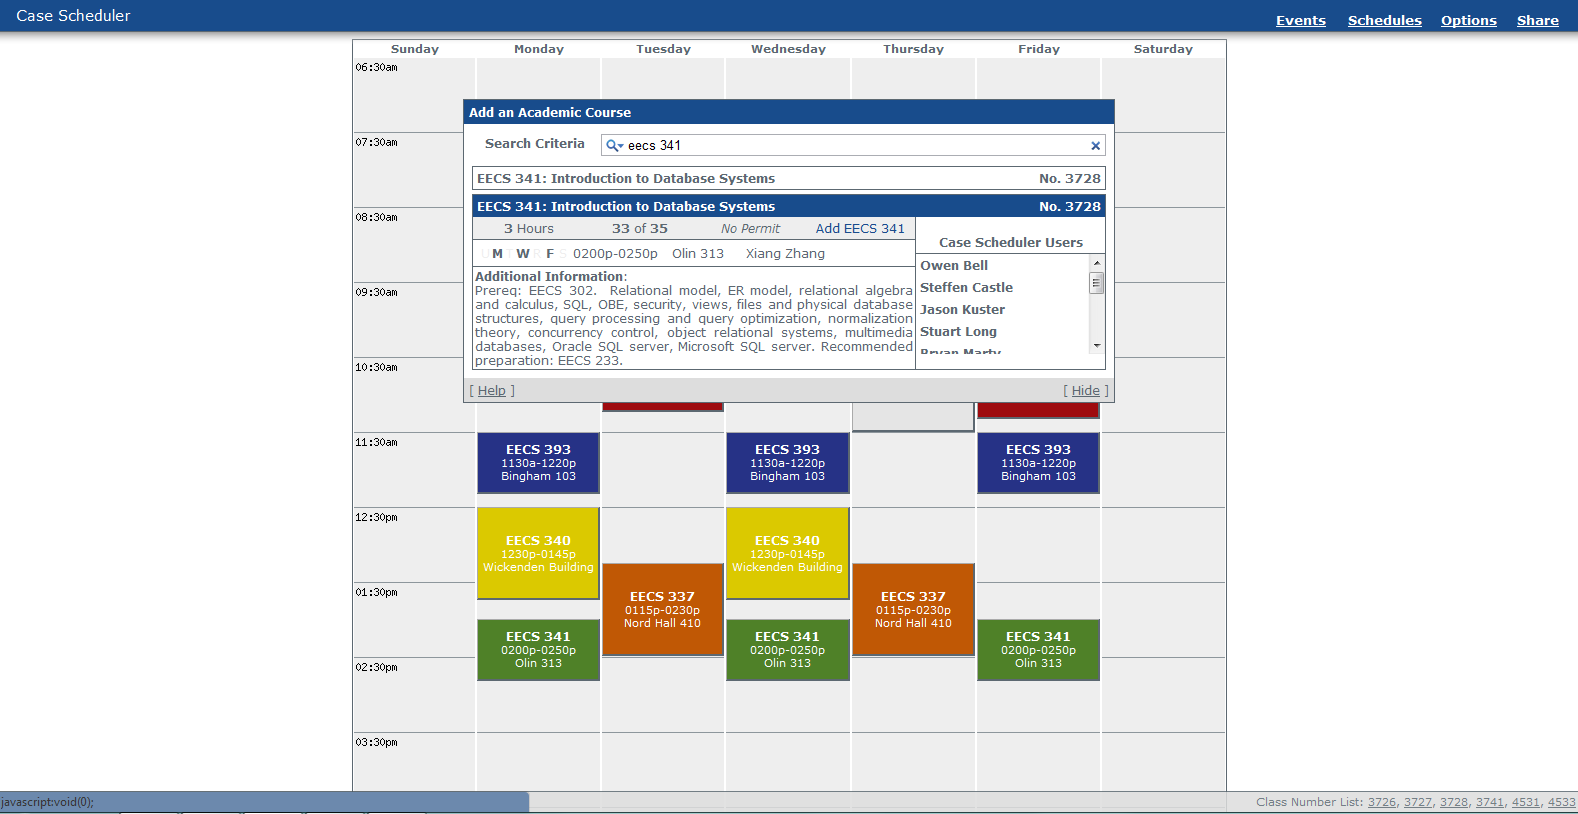
\includegraphics[width=130mm]{add_course.png}
\item The system will allow courses to be added to users' active schedule.\\\\
Once found, a course must be able to be added to a user's currently active schedule. It should stay there until removed either by them or by the system. The functionality of this will be very similar to the functionality of the current Case Scheduler, as shown in the above graphic, but will have a reworked user interface designed by our team.
\item The system should support removing a course from a particular schedule.\\\\
As a user's courses can change during the planning stages or during drop/add, users should be able to remove courses which they have added from their lists.
\item The system will display course information on a weekly calendar-formatted schedule, including course name, times, instructor, and location.\\\\
This format seems to be the easiest and most convenient to view, and gives users a quick and easy-to-use overview of their courses for the week. In the future, other layouts such as a list-type view, day-by-day view, and monthly view. Our implementation of the weekly view will look similar to the below graphic, although with a rewritten user interface backend.\\
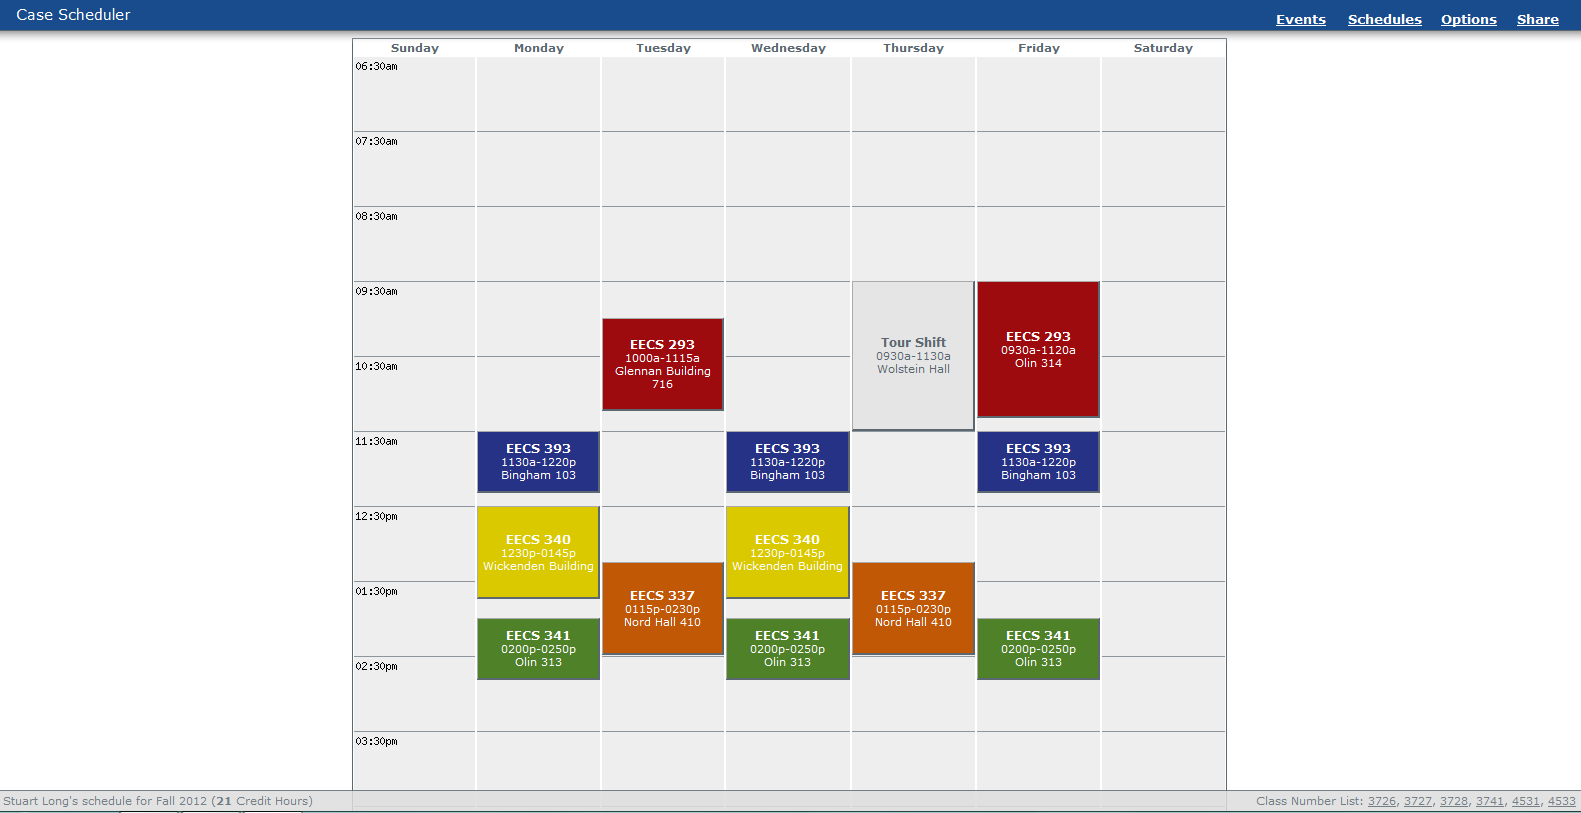
\includegraphics[width=130mm]{main_schedule.png}
\item The system should display itself in a manner which facilitates printing.\\\\
The current system makes it exceedingly difficult to print one's schedule. We are making sure that by design our system will be formatted for printing without users having to do anything.
\item The system should maintain users' lists across SIS updates.\\\\
As the list of courses is subject to change as courses are added or removed in SIS, we will make sure that our application remains robust across these changes and that when responding to changes in the schedule of classes xml file, we do not inadvertently break anyone's schedule.
\item Clicking on courses will bring up more detailed course information.\\\\
As there is a wealth of information about the courses in SIS, we plan to make that data consumable by our users by adding a detail page to each course. This detail page will include such items as classroom, teacher, and meeting times, among others.
\item Under reasonable load, the system should have loading times of less than one second.\\\\
At the current time, scheduler.case.edu can take upwards of 15 seconds to properly aggregate and display all of a user's classes. This frustrates users and is a design flaw which should be easily remediable. Our system will have much faster response times, ensuring greater user satisfaction and a more usable product.
\item The system will allow users to change their current working semester, and will maintain schedules up to 4 years in the past.\\\\
This is necessary in order to allow users to plan a next semester while having a schedule for their current semester. The second SIS data is available, we will make it available to the students and allow them to start planning their next semester. In addition, the ability to go and see what courses they have taken in previous semesters provides value because students will no longer have to do the time-consuming process of using SIS.
\item The system supports the creation of custom events.\\\\
In order to be a one-stop schedule manager, as well as to remain more feature-complete than the current case scheduler, we will be adding support for custom events such as TA sessions, jobs, and other user-defined events. These custom events will have all of the behavior of courses, but will be visible only to their creator, i.e they will not appear in searches. The add dialog will look similar to below.\\
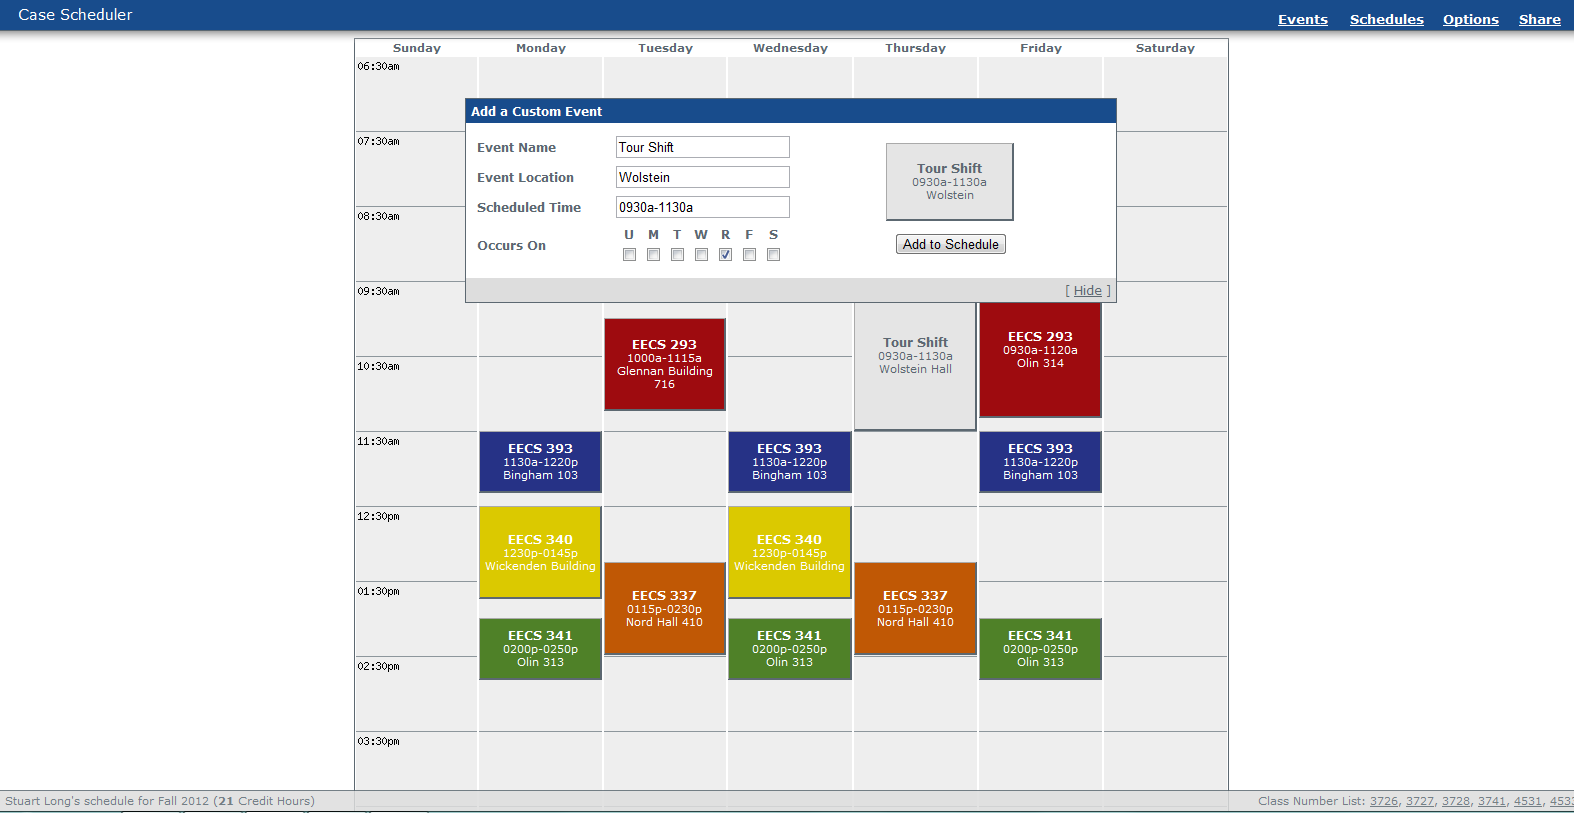
\includegraphics[width=130mm]{add_event.png}
\end{enumerate}
\section*{Database Requirements Specifications}
\subsection*{Objects and Relationships}
\begin{enumerate}[1.]
\item Course Offering: The database will have an instance of course offering for each course offered by CWRU. We considered having a overreaching "Course" object where Course Offering is-a Course. However since the purpose of our application is mainly as a scheduler we are more concerned with attribute specific to each offering, namely when the course is held, we decided to just have the course offering. A course offering will have at least the following attributes: offering id, term, subject, catalog number, title, label, component, status, dates, units (max), days/times, room, total capacity, current enrollment, prerequisites, and description.\\\\ In explanation, the "label" attribute corresponds to a short combination of the of the subject, catalog number, and title. The catalog number corresponds to the course number within that courses department (e.g. 314 for EECS 341). The "component" attribute represents the type of the course, whether it's a lecture, recitation, or similar. The "status" attribute represents whether the course is  open, closed, or other. "Current Enrollment" signifies how many other students are registered for the course offering. "Description" is a paragraph explanation of the course provided by the department or professor.
\item User: Every user will log onto our application with their case id and password (using the single sign on service as provided by CWRU). This process allows us to keep an object representation of each user. This application doesn't need much information about each user, so it will just keep track of the user's case id and last login date. We keep track of their login date so we can safely delete a user and any relationships that user participated in after the user has not logged in for four years.
\item Instructor: Our application will allows users to find basic information about CWRU instructors, such as office location, office hours, and contact information. To adequately display this information, the instructor object will have at least the following attributes: instructor ID, office location, office hours, phone number, and email.
\item Teaches Relationship: Every course offering will be taught by an instance of instructor, and this relation models that, simply by storing the id's for the course offering and the instructor that teaches it. We assume a course offering is not taught by more than one instructor, an assumption that is sufficient for a scheduling application.
\item Enrolled-in Relationship: Multiple students can take multiple different courses, and courses can have many students enrolled in it, up to that courses capacity. This relationship is fairly simple in that it just keeps track of a student and a course that student is enrolled in. However, it is also an extremely important relationship because it allows us to populate a students schedule.
\end{enumerate}
\subsection*{Queries and Transactions}
\begin{enumerate}[1.]
\item Get\_List Query - Very frequent, once ppv
\item Lookup\_Course - Even more frequent, multiples times ppv
\item Add\_Course - Less frequent, less than once ppv
\item Remove\_Course - Infrequent, much less than once ppv
\item Lookup\_Instructor - Infrequent, less than 1 in 10 pv's
\end{enumerate}
\subsection*{Actions and Events}
\begin{enumerate}[1.]
\item This application will display users' schedule based on the currently selected semester, with the default semester being the current semester at the time of the user login. The application will have a drop down list or similar form that will allow users' to select any other schedule in which the user has a course. As can be seen above, the database does not have an actual "schedule" object. To craft various semester schedules, the course offering relations will just be queried for term and the user's schedules will be constructed off of that. All of a user's schedules will be stored until that user is deleted, see \textit{Integrity Constraints} for user deletion policies.
\item An event that will happen every time the application is used by any user is a user login. To use this application a user must have a CWRU ID and password, and will log in with the CWRU Single Sign-On Service. By logging in, the application will be able to identify the user and load all of that user's schedules.
\end{enumerate}
\subsection*{Integrity Constraints}
\begin{enumerate}
\item Users must be enrolled in at least one course offering. If, for some reason, a user is no longer enrolled in any course offering, then that user is removed from the database. If the user wants to use an application after being deleted, than a new "user" object for that user will be created upon log-in, as if that user was a first time user.
\item This application may have to handle up to all CWRU community members and several schedules per user. In order to maintain a flexible ceiling on the database, users that have been inactive for more than four years. If a user is removed and one of the course offerings that that user was enrolled in no longer has any users enrolled in it, then that course offering is deleted as well.
\item If, at any time, a course offering has no users enrolled in it, and the current semester is after the semester that course offering took place in, then that course offering will be removed.
\item Instructors are allowed to not teach a course offering at any given time. However, if an instructor continuously does not teach a course for five years, then that instructor is removed.
\end{enumerate}

\end{document}
